\begin{surferPage}{An $A_4^{+-}$ Singularity}
An $A_4^{+-}$ singularity looks very similar to any singularity of type
    $A_{2k}^{+-}$, $k\ge 1$, as we can see by considering the equation:
    \[x^{2k+1}+y^2-z^2=0.\]
    The only difference to the $A_2^{+-}$ singularity (leftmost picture below)
    is the order of tangency. 
    The middle and rightmost picture show singularities of type $A_4^{+-}$ and
    $A_6^{+-}$), respectively: 
    \vspace*{-0.5em}
    \begin{center}
      \begin{tabular}{c@{\quad}c@{\quad}c}
        \begin{tabular}{@{}c@{}}
          
\includegraphics[width=1.2cm]{../../common/images/A2pm}
        \end{tabular}
        &
        \begin{tabular}{@{}c@{}}
          
\includegraphics[width=1.2cm]{../../common/images/A4pm}
        \end{tabular}
        &
        \begin{tabular}{@{}c@{}}
          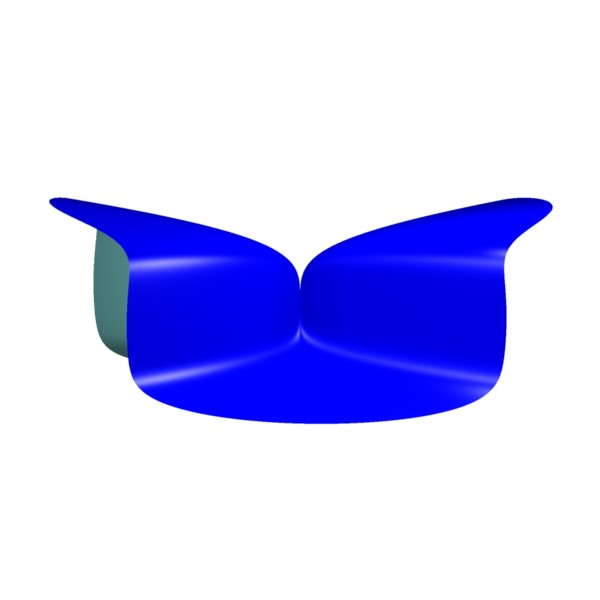
\includegraphics[width=1.2cm]{../../common/images/A6pm}
        \end{tabular}
      \end{tabular}
    \end{center}
    \vspace*{-0.4em}
    However, we recognize a major difference when trying to deform the
    singularity into may double cones. 
    We do not show this here; instead we consider a similar deformation into
    a surface with many holes:
    For an $A_k^{+-}$ singularity we may obtain $k$ holes (here, $k=4$: two
    holes can be seen from 
    each side, see picture below) instead of the two for the $A_2^{+-}$ singularity:
    \begin{center}
      \vspace{-0.1cm}
      \begin{tabular}{@{}c@{\quad}c@{}}
        \begin{tabular}{@{}c@{}}
          
\includegraphics[width=1.2cm]{../../common/images/A4pm_sm_0}
        \end{tabular}
        &
        \begin{tabular}{@{}c@{}}
          
\includegraphics[width=1.2cm]{../../common/images/A4pm_sm_1}
        \end{tabular}
      \end{tabular}
    \end{center}
%     \dontshow{
%     % 
%     \begin{center}
%       \vspace{-0.1cm}
%       \begin{tabular}{@{}c@{\quad}c@{\quad}c@{}}
%         \begin{tabular}{@{}c@{}}
%           
\includegraphics[width=1.2cm]{../../common/images/A4pm_0}
%         \end{tabular}
%         &
%         \begin{tabular}{@{}c@{}}
%           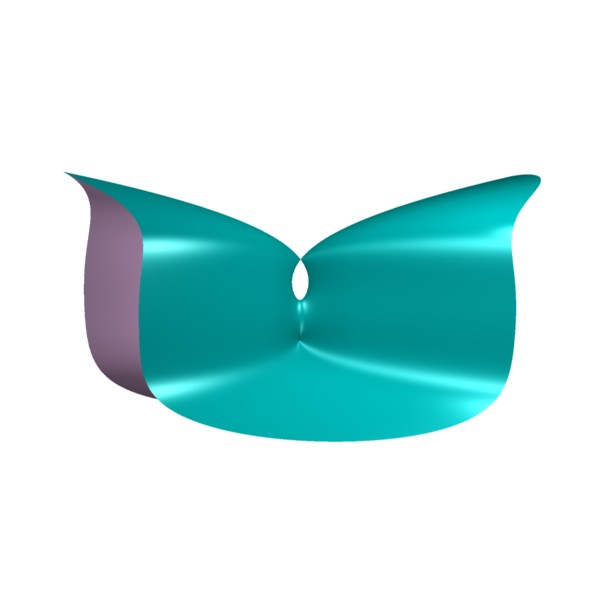
\includegraphics[width=1.2cm]{../../common/images/A4pm_1}
%         \end{tabular}
%         &
%         \begin{tabular}{@{}c@{}}
%           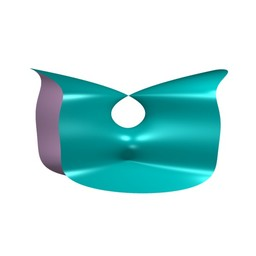
\includegraphics[width=1.2cm]{../../common/images/A4pm_2}
%         \end{tabular}
%       \end{tabular}
%     \end{center}
%     }
 
\end{surferPage}

